\chapter{Advanced JavaFX}

\section{Model-View-Controller (MVC)}

Model-View-Controller (MVC) adalah pola arsitektur yang memisahkan logika bisnis, tampilan, dan interaksi pengguna ke dalam tiga komponen utama. Model bertanggung jawab untuk mengelola data dan logika bisnis, View bertugas untuk menampilkan informasi kepada pengguna, dan Controller menghubungkan interaksi pengguna dengan model serta memperbarui tampilan. Penerapan MVC dalam JavaFX memungkinkan pemisahan yang jelas antara komponen-komponen tersebut, meningkatkan modularitas serta mempermudah pemeliharaan dan pengembangan aplikasi lebih lanjut.

Diagram berikut menggambarkan pola arsitektur Model-View-Controller (MVC), yang sering digunakan dalam pengembangan perangkat lunak, terutama dalam framework seperti JavaFX. MVC memisahkan logika bisnis, antarmuka pengguna, dan kontrol aliran data dalam aplikasi, yang membuatnya lebih mudah dikelola dan diperluas.

\begin{figure}[ht]
	\centering
	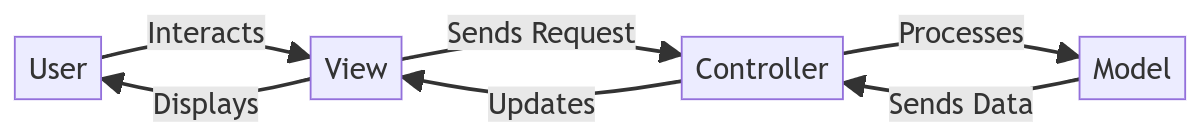
\includegraphics[width=\textwidth]{../figures/mvc-modern.png}
	\caption{Model View Controller Architecture}
	\label{fig:mvc_architecture}
\end{figure}

Pengguna berinteraksi dengan aplikasi melalui antarmuka pengguna yang dikenal sebagai View. View mencakup elemen-elemen seperti tombol, formulir, tabel, dan komponen visual lainnya yang memungkinkan pengguna memberikan input dan menerima output dari aplikasi. Sebagai contoh, dalam JavaFX, pengguna dapat mengklik tombol "Submit" pada sebuah formulir untuk memulai suatu aksi.

Ketika pengguna melakukan suatu aksi pada View, seperti mengklik tombol atau memasukkan teks, View akan mengirimkan permintaan tersebut ke Controller. View tidak menangani logika pemrosesan sendiri, melainkan menyerahkan tugas tersebut kepada Controller. Dalam JavaFX, View dapat memicu metode di Controller melalui event handler seperti \texttt{onAction} pada sebuah tombol.

Controller menerima permintaan dari View dan kemudian memprosesnya dengan berinteraksi dengan Model. Model adalah komponen yang bertanggung jawab atas logika bisnis dan operasi data, seperti mengakses database, melakukan perhitungan, atau memanipulasi data aplikasi. Sebagai contoh, Controller dapat memanggil metode di Model untuk mendapatkan daftar produk dari database.

Setelah Model selesai memproses permintaan, Model akan mengirimkan data kembali ke Controller. Data ini bisa berupa hasil query dari database, hasil perhitungan, atau data yang telah diproses sesuai logika bisnis. Dalam JavaFX, Model mungkin mengembalikan daftar objek yang kemudian dapat digunakan oleh Controller untuk memperbarui tampilan aplikasi.

Controller kemudian mengambil data dari Model dan memperbarui View sesuai dengan data tersebut. Pembaruan ini mungkin melibatkan pengisian tabel dengan data baru, memperbarui teks di label, atau menampilkan notifikasi kepada pengguna. Sebagai contoh, Controller di JavaFX dapat memperbarui elemen \texttt{TableView} dengan data terbaru yang diterima dari Model.

Terakhir, View akan menampilkan data yang telah diperbarui kepada pengguna. Pengguna kemudian dapat melihat hasil dari aksi yang mereka lakukan sebelumnya, seperti melihat tabel produk yang sudah terisi dengan data terbaru. Proses ini menciptakan siklus interaksi antara pengguna dan aplikasi, di mana setiap aksi pengguna dapat memicu pembaruan View melalui Controller dan Model.


\section{Prasyarat Java dan MySQL}
Sebelum memulai pengembangan aplikasi JavaFX, pastikan bahwa perangkat lunak berikut telah terinstal:

\begin{itemize}
	\item Java Development Kit (JDK) minimal versi 11 atau lebih baru.
	\item MySQL sebagai basis data untuk penyimpanan data aplikasi.
	\item Driver JDBC MySQL agar Java dapat berkomunikasi dengan database.
	\item Gradle sebagai build tool untuk mengelola dependensi dan otomasi proses pembangunan proyek.
\end{itemize}

\section{Mengunduh dan Menginstal Gradle serta Konfigurasi Proyek Java dengan Gradle}

Gradle adalah alat otomatisasi pembangunan proyek yang banyak digunakan dalam pengembangan perangkat lunak modern. Untuk menginstalnya, unduh versi terbaru dari situs resmi Gradle dan pastikan variabel lingkungan telah dikonfigurasi dengan benar agar dapat diakses melalui terminal. Untuk menginstal Gradle di sistem berbasis Linux, ikuti pentunjuk pada tautan berikut \url{https://gradle.org/install/}.


Langkah-langkah untuk menginisialisasi proyek Java dengan Gradle:

\begin{enumerate}
\item Pastikan Gradle telah terinstal dengan menjalankan perintah berikut:
\begin{lstlisting}[language=bash]
gradle -v
\end{lstlisting}

\item Buat direktori proyek baru dan masuk ke dalamnya:
\begin{lstlisting}[language=bash]
mkdir my-java-project
cd my-java-project
\end{lstlisting}

\item Jalankan perintah berikut untuk menginisialisasi proyek Java dengan Gradle:
\begin{lstlisting}[language=bash]
gradle init --type java-application
\end{lstlisting}
\end{enumerate}

Dengan perintah di atas, Gradle akan langsung menginisialisasi proyek Java sebagai aplikasi, tanpa perlu memilih opsi secara manual. Proyek Java dengan Gradle telah berhasil dikonfigurasi dan siap digunakan untuk pengembangan aplikasi berbasis Java.

\section{Struktur Direktori Proyek}
Setelah Gradle dikonfigurasi, target \texttt{folder} dan \texttt{files} yang akan dibuat dalam proyek ini adalah sebagai berikut.

\begin{lstlisting}[language=bash]
	my-javafx-project/
	|-- app/
	|   |-- build.gradle
	|   |-- src/
	|   |   |-- main/
	|   |   |   |-- java/
	|   |   |   |   |-- org/example/controllers/
	|   |   |   |   |   |-- ItemController.java
	|   |   |   |   |   |-- MainController.java
	|   |   |   |   |   |-- SalesOrderController.java
	|   |   |   |   |   |-- SelectFormController.java
	|   |   |   |   |-- org/example/helpers/
	|   |   |   |   |   |-- IForm.java
	|   |   |   |   |-- org/example/models/
	|   |   |   |   |   |-- Item.java
	|   |   |   |   |   |-- Order.java
	|   |   |   |   |   |-- OrderDetail.java
	|   |   |   |   |   |-- OrderDetailPK.java
	|   |   |   |-- resources/
	|   |   |   |   |-- hibernate.cfg.xml
	|   |   |   |   |-- Item.fxml
	|   |   |   |   |-- Main.fxml
	|   |   |   |   |-- SalesOrder.fxml
	|   |   |   |   |-- SelectForm.fxml
	|   |   |   |   |-- test.rptdesign
	|-- settings.gradle
	|-- gradle.properties
	|-- gradlew
	|-- gradlew.bat
\end{lstlisting}


Struktur proyek JavaFX ini terdiri dari beberapa direktori dan file utama yang dikelompokkan berdasarkan fungsinya. Berikut adalah target direktori dan file yang digunakan dalam proyek ini:

\begin{enumerate}
	\item \textbf{Root Direktori}:
	\begin{itemize}
		\item \texttt{settings.gradle} - File konfigurasi Gradle yang mengatur pengelolaan proyek multi-modul.
		\item \texttt{gradle.properties} - File properti Gradle yang menyimpan konfigurasi global proyek.
		\item \texttt{gradlew} dan \texttt{gradlew.bat} - Skrip untuk menjalankan Gradle Wrapper di sistem Unix dan Windows.
	\end{itemize}
	
	\item \textbf{Direktori Aplikasi (app/)}:
	\begin{itemize}
		\item \texttt{build.gradle} - File konfigurasi Gradle yang mengelola dependensi dan pengaturan proyek aplikasi.
		\item \texttt{src/} - Direktori utama yang berisi kode sumber proyek.
	\end{itemize}
	
	\item \textbf{Direktori Kode Sumber (src/main/)}:
	\begin{itemize}
		\item \texttt{java/org/example/controllers/} - Berisi kelas \textbf{Controller} yang menangani logika aplikasi, seperti \texttt{ItemController.java}, \texttt{MainController.java}, dan lainnya.
		\item \texttt{java/org/example/helpers/} - Berisi kelas bantuan yang mendukung operasi aplikasi, seperti \texttt{IForm.java}.
		\item \texttt{java/org/example/models/} - Berisi \textbf{Model} data yang merepresentasikan entitas bisnis, seperti \texttt{Item.java}, \texttt{Order.java}, dan \texttt{OrderDetail.java}.
	\end{itemize}
	
	\item \textbf{Direktori Resource (src/main/resources/)}:
	\begin{itemize}
		\item \texttt{hibernate.cfg.xml} - Konfigurasi Hibernate untuk menghubungkan aplikasi dengan database.
		\item Berkas \textbf{View} JavaFX dalam format \texttt{FXML}, seperti \texttt{Item.fxml}, \texttt{Main.fxml}, \texttt{SalesOrder.fxml}, dan \texttt{SelectForm.fxml}.
		\item \texttt{test.rptdesign} - Template laporan yang digunakan dalam aplikasi.
	\end{itemize}
\end{enumerate}


\section{Konfigurasi Gradle}

File \texttt{build.gradle} dalam proyek ini mengatur konfigurasi build menggunakan Gradle. Berikut adalah kode lengkap yang digunakan dalam file tersebut:

\begin{lstlisting}[style=JavaStyle]
	plugins {
		id 'application'
		id 'org.openjfx.javafxplugin' version '0.1.0'
	}
	
	repositories {
		mavenCentral()
	}
	
	dependencies {
		implementation 'mysql:mysql-connector-java:8.0.33'
		implementation 'org.hibernate:hibernate-core:6.2.12.Final'
		implementation 'jakarta.persistence:jakarta.persistence-api:3.1.0'
		implementation "org.openjfx:javafx-controls:20.0.1"
		implementation "org.openjfx:javafx-fxml:20.0.1"
		implementation 'com.innoventsolutions.birt.runtime:org.eclipse.birt.runtime_4.8.0-20180626:4.8.0'
		
		testImplementation libs.junit.jupiter
		testRuntimeOnly 'org.junit.platform:junit-platform-launcher'
		implementation libs.guava
	}
	
	java {
		toolchain {
			languageVersion = JavaLanguageVersion.of(21)
		}
	}
	
	application {
		mainClass = 'org.example.Main'
	}
	
	tasks.named('test') {
		useJUnitPlatform()
	}
	
	javafx {
		version = "21.0.1"
		modules = [ 'javafx.controls', 'javafx.fxml' ]
	}
\end{lstlisting}

Bagian \texttt{plugins} mendefinisikan plugin yang digunakan dalam proyek. Plugin \texttt{application} digunakan untuk aplikasi Java biasa, sedangkan \texttt{org.openjfx.javafxplugin} digunakan untuk mendukung JavaFX.

Bagian \texttt{repositories} menentukan lokasi tempat dependensi akan diunduh. Dalam konfigurasi ini, proyek menggunakan \texttt{mavenCentral()} sebagai repositori utama.

Bagian \texttt{dependencies} mendefinisikan pustaka eksternal yang digunakan dalam proyek. MySQL Connector digunakan untuk koneksi ke database MySQL. Hibernate Core digunakan untuk Object-Relational Mapping (ORM) dan manajemen database. Jakarta Persistence API merupakan API standar untuk ORM berbasis Java. JavaFX Controls dan JavaFX FXML menyediakan komponen antarmuka pengguna untuk JavaFX. BIRT Runtime digunakan untuk rendering laporan dalam aplikasi. JUnit dan Guava digunakan untuk pengujian unit dan utilitas tambahan dalam Java.

Bagian \texttt{java.toolchain} memastikan bahwa proyek menggunakan Java 21 sebagai versi bahasa pemrograman yang dikompilasi. Bagian \texttt{application} mendefinisikan kelas utama yang akan dijalankan dalam aplikasi, dalam hal ini \texttt{org.example.Main}. Bagian \texttt{tasks.named('test')} mengonfigurasi Gradle untuk menggunakan JUnit Platform sebagai framework pengujian. Bagian \texttt{javafx} menentukan versi JavaFX yang digunakan serta modul yang diperlukan dalam aplikasi.

\section{Konfigurasi Hibernate}

File \texttt{hibernate.cfg.xml} digunakan untuk mengonfigurasi Hibernate sebagai ORM (Object-Relational Mapping) yang menghubungkan aplikasi Java dengan database MySQL. Berikut adalah kode konfigurasi yang digunakan:

\begin{lstlisting}[style=XmlStyle]
	<?xml version="1.0" encoding="utf-8"?>
	<!DOCTYPE hibernate-configuration PUBLIC 
	"-//Hibernate/Hibernate Configuration DTD 3.0//EN"
	"http://www.hibernate.org/dtd/hibernate-configuration-3.0.dtd">
	<hibernate-configuration>
	<session-factory>
	<!-- Database Configuration -->
	<property name="hibernate.connection.driver_class">com.mysql.cj.jdbc.Driver</property>
	<property name="hibernate.connection.url">jdbc:mysql://localhost:3306/pradita?useSSL=false&amp;serverTimezone=UTC</property>
	<property name="hibernate.connection.username">alfa</property>
	<property name="hibernate.connection.password">1234</property>
	
	<!-- Hibernate Settings -->
	<property name="hibernate.dialect">org.hibernate.dialect.MySQLDialect</property>
	<property name="hibernate.show_sql">true</property>
	<property name="hibernate.format_sql">true</property>
	<property name="hibernate.hbm2ddl.auto">update</property>
	
	<!-- Entity Mappings -->
	<mapping class="org.example.models.Order"/>
	<mapping class="org.example.models.OrderDetail"/>
	<mapping class="org.example.models.Item"/>
	</session-factory>
	</hibernate-configuration>
\end{lstlisting}

Konfigurasi ini terdiri dari beberapa bagian utama yang mengatur koneksi database, konfigurasi Hibernate, dan pemetaan entitas.

Bagian pertama adalah pengaturan koneksi ke database MySQL, termasuk driver yang digunakan, URL koneksi, username, dan password. Database yang digunakan dalam konfigurasi ini adalah \texttt{pradita} yang berada di \texttt{localhost} dengan timezone UTC dan tanpa SSL. Parameter \texttt{hibernate.connection.driver\_class} menentukan driver JDBC untuk MySQL. \texttt{hibernate.connection.url} berisi alamat database, sedangkan \texttt{hibernate.connection.username} dan \texttt{hibernate.connection.password} digunakan untuk autentikasi koneksi.

Bagian berikutnya adalah pengaturan Hibernate yang mencakup beberapa properti utama. \texttt{hibernate.dialect} menentukan dialect SQL yang digunakan, dalam hal ini \texttt{MySQLDialect}, agar Hibernate dapat menghasilkan query yang sesuai dengan MySQL. \texttt{hibernate.show\_sql} diatur ke \texttt{true} agar semua query SQL yang dieksekusi dapat dilihat di log, sedangkan \texttt{hibernate.format\_sql} digunakan untuk menampilkan query dalam format yang lebih rapi. Opsi \texttt{hibernate.hbm2ddl.auto} diset ke \texttt{update}, yang memungkinkan Hibernate secara otomatis menyesuaikan struktur tabel database dengan entitas Java.

Bagian terakhir adalah pemetaan entitas yang menentukan kelas-kelas model dalam paket \texttt{org.example.models} yang akan dikelola oleh Hibernate. Konfigurasi ini mencakup tiga kelas utama, yaitu \texttt{Order}, \texttt{OrderDetail}, dan \texttt{Item}. Dengan pengaturan ini, Hibernate dapat menghubungkan kelas-kelas model dengan tabel dalam database secara otomatis dan melakukan operasi CRUD tanpa perlu menulis query SQL manual.

\section{Models}
Dalam arsitektur perangkat lunak berbasis Model-View-Controller (MVC), \textbf{Model} berperan sebagai representasi data dan logika bisnis yang berinteraksi langsung dengan database. Model bertanggung jawab untuk menyimpan, mengelola, dan memanipulasi data yang digunakan dalam aplikasi. Dengan menggunakan Hibernate sebagai ORM (Object-Relational Mapping), setiap entitas dalam model dipetakan ke dalam tabel database, memungkinkan operasi \textbf{CRUD (Create, Read, Update, Delete)} dilakukan secara efisien tanpa perlu menulis query SQL secara manual. Setiap model dalam aplikasi didefinisikan sebagai kelas Java dengan anotasi \texttt{jakarta.persistence} untuk mendeklarasikan hubungan antara atribut dalam kode dengan kolom dalam tabel database. Bagian ini akan membahas berbagai entitas dalam aplikasi, termasuk \texttt{Item}, \texttt{Order}, dan \texttt{OrderDetail}, serta bagaimana masing-masing kelas diimplementasikan dalam Hibernate.

\subsection{Item.java}

File \texttt{Item.java} merupakan kelas entitas yang dipetakan ke tabel \texttt{item} dalam database menggunakan Hibernate. Berikut adalah kode sumbernya:

\begin{lstlisting}[style=JavaStyle]
	package org.example.models;
	
	import jakarta.persistence.Column;
	import jakarta.persistence.Entity;
	import jakarta.persistence.Id;
	import jakarta.persistence.Table;
	
	@Entity
	@Table(name = "item")
	public class Item {
		@Id
		@Column(name = "code", length = 5, nullable = false)
		private String code;
		
		@Column(name = "name", length = 50)
		private String name;
		
		@Column(name = "price", nullable = false)
		private Double price;
		
		@Column(name = "quantity", nullable = false)
		private Double quantity;
		
		// Getters and setters
		public String getCode() { return code; }
		public void setCode(String code) { this.code = code; }
		
		public String getName() { return name; }
		public void setName(String name) { this.name = name; }
		
		public Double getPrice() { return price; }
		public void setPrice(Double price) { this.price = price; }
		
		public Double getQuantity() { return quantity; }
		public void setQuantity(Double quantity) { this.quantity = quantity; }
	}
\end{lstlisting}

Kelas \texttt{Item} menggunakan beberapa anotasi dari \texttt{jakarta.persistence} yang memungkinkan Hibernate untuk memetakan objek Java ke tabel database. \textbf{Setiap anotasi memiliki fungsi spesifik} dalam proses ORM (Object-Relational Mapping) yang dilakukan oleh Hibernate.

\begin{enumerate}
	\item \textbf{Anotasi \texttt{@Entity}}. 
	Anotasi \texttt{@Entity} menandakan bahwa kelas ini merupakan entitas yang akan dipetakan ke dalam tabel database. Hibernate akan mengelola objek dari kelas ini dan menyimpannya dalam database.
	
	\item \textbf{Anotasi \texttt{@Table(name = \"item\")}}. 
	Anotasi \texttt{@Table(name = "item")} mengaitkan kelas \texttt{Item} dengan tabel \texttt{item} dalam database. Jika anotasi ini tidak diberikan, secara default Hibernate akan menggunakan nama kelas sebagai nama tabel.
	
	\item \textbf{Anotasi \texttt{@Id}}. 
	Atribut \texttt{code} digunakan sebagai primary key dari tabel \texttt{item}. Anotasi \texttt{@Id} menandakan bahwa atribut ini adalah kolom unik yang digunakan oleh Hibernate untuk mengidentifikasi setiap entitas dalam database.
	
	\item \textbf{Anotasi \texttt{@Column}}.
	Anotasi \texttt{@Column} digunakan untuk mendefinisikan properti yang akan dipetakan ke dalam kolom tabel database:
	\begin{enumerate}
		\item \texttt{@Column(name = "code", length = 5, nullable = false)} - Kolom \texttt{code} memiliki panjang maksimum 5 karakter dan tidak boleh kosong (\texttt{nullable = false}). Properti ini berfungsi sebagai primary key.
		\item \texttt{@Column(name = "name", length = 50)} - Kolom \texttt{name} memiliki panjang maksimum 50 karakter. Tidak ada batasan \texttt{nullable}, sehingga dapat diisi atau dibiarkan kosong.
		\item \texttt{@Column(name = "price", nullable = false)} - Kolom \texttt{price} menggunakan tipe data \texttt{Double} dan wajib diisi (\texttt{nullable = false}).
		\item \texttt{@Column(name = "quantity", nullable = false)} - Kolom \texttt{quantity} juga menggunakan tipe data \texttt{Double} dan wajib diisi (\texttt{nullable = false}).
	\end{enumerate}
	
	\item \textbf{Penggunaan Getter dan Setter}.
	Setiap atribut memiliki metode getter dan setter. Hibernate membutuhkan metode ini untuk membaca dan memperbarui nilai dari setiap atribut saat melakukan operasi database.

\end{enumerate}

Dengan konfigurasi ini, Hibernate akan melakukan pemetaan tabel \texttt{item} sebagai berikut:
\begin{enumerate}
	\item Setiap objek \texttt{Item} akan diperlakukan sebagai satu baris data dalam tabel \texttt{item}.
	\item Jika sebuah objek \texttt{Item} disimpan menggunakan Hibernate, maka Hibernate akan mengeksekusi query \texttt{INSERT} ke dalam database.
	\item Jika sebuah objek \texttt{Item} diubah, Hibernate akan secara otomatis menjalankan query \texttt{UPDATE} untuk menyimpan perubahan tersebut.
	\item Jika sebuah objek \texttt{Item} dihapus, Hibernate akan menjalankan query \texttt{DELETE}.
\end{enumerate}

Sebagai contoh, ketika kita menyimpan objek baru menggunakan Hibernate:

\begin{lstlisting}[style=JavaStyle]
	Session session = HibernateUtil.getSessionFactory().openSession();
	Transaction transaction = session.beginTransaction();
	
	Item item = new Item();
	item.setCode("A123");
	item.setName("Laptop");
	item.setPrice(15000000.0);
	item.setQuantity(10.0);
	
	session.save(item);
	transaction.commit();
	session.close();
\end{lstlisting}

Kode di atas akan menyebabkan Hibernate mengeksekusi query berikut dalam database:

\begin{lstlisting}[style=sql]
	INSERT INTO item (code, name, price, quantity) 
	VALUES ('A123', 'Laptop', 15000000.0, 10.0);
\end{lstlisting}

Jika kita ingin mengambil data berdasarkan kode barang:

\begin{lstlisting}[style=JavaStyle]
	Session session = HibernateUtil.getSessionFactory().openSession();
	Item item = session.get(Item.class, "A123");
	System.out.println("Nama Barang: " + item.getName());
	session.close();
\end{lstlisting}

Hibernate akan menerjemahkannya ke dalam query SQL berikut:

\begin{lstlisting}[style=sql]
	SELECT * FROM item WHERE code = 'A123';
\end{lstlisting}

Dengan pemetaan ini, Hibernate dapat menangani interaksi dengan database secara otomatis tanpa perlu menulis query SQL secara manual. Hal ini membuat pengelolaan database lebih efisien dan mengurangi ketergantungan pada query SQL yang eksplisit.


\subsection{Order.java}

File \texttt{Order.java} merupakan kelas entitas yang dipetakan ke tabel \texttt{order} dalam database menggunakan Hibernate. Kelas ini berfungsi sebagai model yang merepresentasikan pesanan dalam aplikasi. Berikut adalah kode sumbernya:

\begin{lstlisting}[style=JavaStyle]
	package org.example.models;
	
	import java.time.LocalDateTime;
	import java.util.List;
	
	import jakarta.persistence.CascadeType;
	import jakarta.persistence.Column;
	import jakarta.persistence.Entity;
	import jakarta.persistence.Id;
	import jakarta.persistence.OneToMany;
	import jakarta.persistence.Table;
	
	@Entity
	@Table(name = "order")
	public class Order {
		@Id
		@Column(name = "code", length = 5, nullable = false)
		private String code;
		
		@Column(name = "note", columnDefinition = "TEXT")
		private String note;
		
		@Column(name = "date", columnDefinition = "DATETIME DEFAULT CURRENT_TIMESTAMP")
		private LocalDateTime date;
		
		@OneToMany(mappedBy = "order", cascade = CascadeType.ALL, orphanRemoval = true)
		private List<OrderDetail> orderDetails;
		
		// Getters and setters
		public String getCode() { return code; }
		public void setCode(String code) { this.code = code; }
		
		public String getNote() { return note; }
		public void setNote(String note) { this.note = note; }
		
		public LocalDateTime getDate() { return date; }
		public void setDate(LocalDateTime date) { this.date = date; }
		
		public List<OrderDetail> getOrderDetails() { return orderDetails; }
		public void setOrderDetails(List<OrderDetail> orderDetails) { this.orderDetails = orderDetails; }
	}
\end{lstlisting}

Kelas \texttt{Order} menggunakan beberapa anotasi dari \texttt{jakarta.persistence} yang memungkinkan Hibernate untuk memetakan objek Java ke tabel database.

\begin{enumerate}
	\item \textbf{Anotasi \texttt{@Entity}}. 
	Anotasi \texttt{@Entity} menandakan bahwa kelas ini merupakan entitas yang akan dipetakan ke dalam tabel database. Hibernate akan mengelola objek dari kelas ini dan menyimpannya dalam database.
	
	\item \textbf{Anotasi \texttt{@Table(name = "order")}}. 
	Anotasi \texttt{@Table(name = "order")} mengaitkan kelas \texttt{Order} dengan tabel \texttt{order} dalam database. Jika anotasi ini tidak diberikan, secara default Hibernate akan menggunakan nama kelas sebagai nama tabel.
	
	\item \textbf{Anotasi \texttt{@Id}}. 
	Atribut \texttt{code} digunakan sebagai primary key dari tabel \texttt{order}. Anotasi \texttt{@Id} menandakan bahwa atribut ini adalah kolom unik yang digunakan oleh Hibernate untuk mengidentifikasi setiap entitas dalam database.
	
	\item \textbf{Anotasi \texttt{@Column}}.
	Anotasi \texttt{@Column} digunakan untuk mendefinisikan properti yang akan dipetakan ke dalam kolom tabel database:
	\begin{enumerate}
		\item \texttt{@Column(name = "code", length = 5, nullable = false)} - Kolom \texttt{code} memiliki panjang maksimum 5 karakter dan tidak boleh kosong (\texttt{nullable = false}). Properti ini berfungsi sebagai primary key.
		\item \texttt{@Column(name = "note", columnDefinition = "TEXT")} - Kolom \texttt{note} digunakan untuk menyimpan catatan pesanan dalam format teks panjang.
		\item \texttt{@Column(name = "date", columnDefinition = "DATETIME DEFAULT CURRENT\_TIMESTAMP")} - Kolom \texttt{date} menyimpan waktu pembuatan pesanan dengan nilai default \texttt{CURRENT\_TIMESTAMP}.
	\end{enumerate}
	
	\item \textbf{Anotasi \texttt{@OneToMany}}.
	Atribut \texttt{orderDetails} direpresentasikan sebagai daftar (\texttt{List}) yang berisi \texttt{OrderDetail}. 
	\begin{enumerate}
		\item \texttt{@OneToMany(mappedBy = "order", cascade = CascadeType.ALL, orphanRemoval = true)} \\
		Anotasi ini menunjukkan bahwa hubungan antara \texttt{Order} dan \texttt{OrderDetail} adalah **one-to-many**.
		\begin{itemize}
			\item \texttt{mappedBy = "order"} - Menunjukkan bahwa hubungan ini dikendalikan oleh atribut \texttt{order} dalam kelas \texttt{OrderDetail}.
			\item \texttt{cascade = CascadeType.ALL} - Jika entitas \texttt{Order} dibuat, diperbarui, atau dihapus, maka semua \texttt{OrderDetail} yang terkait akan ikut diperbarui atau dihapus.
			\item \texttt{orphanRemoval = true} - Jika sebuah \texttt{OrderDetail} tidak lagi terkait dengan entitas \texttt{Order}, maka entitas tersebut akan dihapus dari database.
		\end{itemize}
	\end{enumerate}
	
	\item \textbf{Penggunaan Getter dan Setter}.
	Setiap atribut memiliki metode getter dan setter. Hibernate membutuhkan metode ini untuk membaca dan memperbarui nilai dari setiap atribut saat melakukan operasi database.
	
\end{enumerate}

Dengan konfigurasi ini, Hibernate akan melakukan pemetaan tabel \texttt{order} sebagai berikut:
\begin{enumerate}
	\item Setiap objek \texttt{Order} akan diperlakukan sebagai satu baris data dalam tabel \texttt{order}.
	\item Jika sebuah objek \texttt{Order} disimpan menggunakan Hibernate, maka Hibernate akan mengeksekusi query \texttt{INSERT} ke dalam database.
	\item Jika sebuah objek \texttt{Order} diubah, Hibernate akan secara otomatis menjalankan query \texttt{UPDATE} untuk menyimpan perubahan tersebut.
	\item Jika sebuah objek \texttt{Order} dihapus, Hibernate akan menjalankan query \texttt{DELETE}.
\end{enumerate}

Sebagai contoh, ketika kita menyimpan objek baru menggunakan Hibernate:

\begin{lstlisting}[style=JavaStyle]
	Session session = HibernateUtil.getSessionFactory().openSession();
	Transaction transaction = session.beginTransaction();
	
	Order order = new Order();
	order.setCode("O123");
	order.setNote("Pesanan pertama");
	order.setDate(LocalDateTime.now());
	
	session.save(order);
	transaction.commit();
	session.close();
\end{lstlisting}

Kode di atas akan menyebabkan Hibernate mengeksekusi query berikut dalam database:

\begin{lstlisting}[style=sql]
	INSERT INTO `order` (code, note, date) 
	VALUES ('O123', 'Pesanan pertama', CURRENT_TIMESTAMP);
\end{lstlisting}

Jika kita ingin mengambil data berdasarkan kode pesanan:

\begin{lstlisting}[style=JavaStyle]
	Session session = HibernateUtil.getSessionFactory().openSession();
	Order order = session.get(Order.class, "O123");
	System.out.println("Catatan Pesanan: " + order.getNote());
	session.close();
\end{lstlisting}

Hibernate akan menerjemahkannya ke dalam query SQL berikut:

\begin{lstlisting}[style=sql]
	SELECT * FROM `order` WHERE code = 'O123';
\end{lstlisting}

Dengan pemetaan ini, Hibernate dapat menangani interaksi dengan database secara otomatis tanpa perlu menulis query SQL secara manual. Konfigurasi ini memastikan bahwa hubungan antara pesanan dan detail pesanan dapat dikelola dengan baik oleh Hibernate.


\subsection{OrderDetail.java}

File \texttt{OrderDetail.java} merupakan kelas entitas yang dipetakan ke tabel \texttt{order\_detail} dalam database menggunakan Hibernate. Kelas ini menyimpan detail pesanan yang terkait dengan pesanan utama dalam aplikasi. Berikut adalah kode sumbernya:

\begin{lstlisting}[style=JavaStyle]
	package org.example.models;
	
	import jakarta.persistence.Column;
	import jakarta.persistence.EmbeddedId;
	import jakarta.persistence.Entity;
	import jakarta.persistence.JoinColumn;
	import jakarta.persistence.ManyToOne;
	import jakarta.persistence.MapsId;
	import jakarta.persistence.Table;
	
	@Entity
	@Table(name = "order_detail")
	public class OrderDetail {
		@EmbeddedId
		private OrderDetailPK id;
		
		@ManyToOne
		@MapsId("orderCode")
		@JoinColumn(name = "code", nullable = false)
		private Order order;
		
		@Column(name = "itemcode", length = 5, nullable = false)
		private String itemCode;
		
		@Column(name = "name", length = 50)
		private String name;
		
		@Column(name = "price", nullable = false)
		private Double price;
		
		@Column(name = "quantity", nullable = false)
		private Double quantity;
		
		public OrderDetail(OrderDetailPK id, Order order, String itemCode, String name, double price, double quantity) {
			this.id = id;
			this.order = order;
			this.itemCode = itemCode;
			this.name = name;
			this.price = price;
			this.quantity = quantity;
		}
		
		// Getters and setters
		public OrderDetailPK getId() { return id; }
		public void setId(OrderDetailPK id) { this.id = id; }
		
		public Order getOrder() { return order; }
		public void setOrder(Order order) { this.order = order; }
		
		public String getItemCode() { return itemCode; }
		public void setItemCode(String itemCode) { this.itemCode = itemCode; }
		
		public String getName() { return name; }
		public void setName(String name) { this.name = name; }
		
		public Double getPrice() { return price; }
		public void setPrice(Double price) { this.price = price; }
		
		public Double getQuantity() { return quantity; }
		public void setQuantity(Double quantity) { this.quantity = quantity; }
	}
\end{lstlisting}

Kelas \texttt{OrderDetail} menggunakan beberapa anotasi dari \texttt{jakarta.persistence} yang memungkinkan Hibernate untuk memetakan objek Java ke tabel database.

\begin{enumerate}
	\item \textbf{Anotasi \texttt{@Entity}}. 
	Anotasi \texttt{@Entity} menandakan bahwa kelas ini merupakan entitas yang akan dipetakan ke dalam tabel database. Hibernate akan mengelola objek dari kelas ini dan menyimpannya dalam database.
	
	\item \textbf{Anotasi \texttt{@Table(name = "order\_detail")}}. 
	Anotasi \texttt{@Table(name = "order\_detail")} mengaitkan kelas \texttt{OrderDetail} dengan tabel \texttt{order\_detail} dalam database.
	
	\item \textbf{Anotasi \texttt{@EmbeddedId}}. 
	Anotasi \texttt{@EmbeddedId} menunjukkan bahwa primary key dari entitas ini terdiri dari beberapa kolom yang dikelola dalam kelas \texttt{OrderDetailPK}.
	
	\item \textbf{Anotasi \texttt{@ManyToOne}}. 
	Anotasi \texttt{@ManyToOne} menunjukkan bahwa entitas ini memiliki relasi **many-to-one** dengan \texttt{Order}, di mana banyak \texttt{OrderDetail} dapat terkait dengan satu \texttt{Order}.
	
	\item \textbf{Anotasi \texttt{@MapsId}}. 
	Anotasi \texttt{@MapsId("orderCode")} menunjukkan bahwa nilai primary key dari \texttt{OrderDetail} akan menggunakan primary key dari \texttt{Order}.
	
	\item \textbf{Anotasi \texttt{@JoinColumn}}. 
	Anotasi \texttt{@JoinColumn(name = "code", nullable = false)} menentukan bahwa kolom \texttt{code} adalah foreign key yang menghubungkan entitas ini dengan tabel \texttt{order}.
	
	\item \textbf{Anotasi \texttt{@Column}}. 
	Anotasi \texttt{@Column} digunakan untuk mendefinisikan properti yang akan dipetakan ke dalam kolom tabel database:
	\begin{enumerate}
		\item \texttt{@Column(name = "itemcode", length = 5, nullable = false)} - Kolom \texttt{itemcode} menyimpan kode item dengan panjang maksimum 5 karakter dan tidak boleh kosong.
		\item \texttt{@Column(name = "name", length = 50)} - Kolom \texttt{name} menyimpan nama item dengan panjang maksimum 50 karakter.
		\item \texttt{@Column(name = "price", nullable = false)} - Kolom \texttt{price} menyimpan harga item dan wajib diisi.
		\item \texttt{@Column(name = "quantity", nullable = false)} - Kolom \texttt{quantity} menyimpan jumlah item dan wajib diisi.
	\end{enumerate}
	
	\item \textbf{Penggunaan Getter dan Setter}. 
	Setiap atribut memiliki metode getter dan setter. Hibernate membutuhkan metode ini untuk membaca dan memperbarui nilai dari setiap atribut saat melakukan operasi database.
\end{enumerate}

Dengan konfigurasi ini, Hibernate akan melakukan pemetaan tabel \texttt{order\_detail} sebagai berikut:
\begin{enumerate}
	\item Setiap objek \texttt{OrderDetail} akan diperlakukan sebagai satu baris data dalam tabel \texttt{order\_detail}.
	\item Jika sebuah objek \texttt{OrderDetail} disimpan menggunakan Hibernate, maka Hibernate akan mengeksekusi query \texttt{INSERT} ke dalam database.
	\item Jika sebuah objek \texttt{OrderDetail} diubah, Hibernate akan secara otomatis menjalankan query \texttt{UPDATE} untuk menyimpan perubahan tersebut.
	\item Jika sebuah objek \texttt{OrderDetail} dihapus, Hibernate akan menjalankan query \texttt{DELETE}.
\end{enumerate}

Sebagai contoh, ketika kita menyimpan objek baru menggunakan Hibernate:

\begin{lstlisting}[style=JavaStyle]
	Session session = HibernateUtil.getSessionFactory().openSession();
	Transaction transaction = session.beginTransaction();
	
	OrderDetailPK id = new OrderDetailPK("O123", "I567");
	Order order = session.get(Order.class, "O123");
	OrderDetail orderDetail = new OrderDetail(id, order, "I567", "Mouse", 50000.0, 2.0);
	
	session.save(orderDetail);
	transaction.commit();
	session.close();
\end{lstlisting}

Kode di atas akan menyebabkan Hibernate mengeksekusi query berikut dalam database:

\begin{lstlisting}[style=sql]
	INSERT INTO order_detail (code, itemcode, name, price, quantity) 
	VALUES ('O123', 'I567', 'Mouse', 50000.0, 2.0);
\end{lstlisting}

Dengan pemetaan ini, Hibernate dapat menangani interaksi dengan database secara otomatis tanpa perlu menulis query SQL secara manual. Konfigurasi ini memastikan bahwa hubungan antara detail pesanan dan pesanan utama dapat dikelola dengan baik oleh Hibernate.


\subsection{OrderDetailPK.java}

File \texttt{OrderDetailPK.java} merupakan kelas yang digunakan sebagai \textbf{primary key} komposit dalam entitas \texttt{OrderDetail}. Kelas ini berfungsi sebagai identifier unik yang terdiri dari beberapa kolom dalam tabel \texttt{order\_detail}. Berikut adalah kode sumbernya:

\begin{lstlisting}[style=JavaStyle]
	package org.example.models;
	
	import java.util.Objects;
	import jakarta.persistence.Column;
	import jakarta.persistence.Embeddable;
	
	@Embeddable
	public class OrderDetailPK implements java.io.Serializable {
		@Column(name = "code", length = 5, nullable = false)
		private String orderCode;
		
		@Column(name = "line", nullable = false)
		private Integer line;
		
		public OrderDetailPK(String newCode, int line) {
			this.orderCode = newCode;
			this.line = line;
		}
		
		// Getters, setters, equals, and hashCode
		public String getOrderCode() { return orderCode; }
		public void setOrderCode(String orderCode) { this.orderCode = orderCode; }
		
		public Integer getLine() { return line; }
		public void setLine(Integer line) { this.line = line; }
		
		@Override
		public boolean equals(Object o) {
			if (this == o)
			return true;
			if (o == null || getClass() != o.getClass())
			return false;
			OrderDetailPK that = (OrderDetailPK) o;
			return orderCode.equals(that.orderCode) && line.equals(that.line);
		}
		
		@Override
		public int hashCode() {
			return Objects.hash(orderCode, line);
		}
	}
\end{lstlisting}

Kelas \texttt{OrderDetailPK} menggunakan beberapa anotasi dari \texttt{jakarta.persistence} yang memungkinkan Hibernate untuk menangani primary key komposit.

\begin{enumerate}
	\item \textbf{Anotasi \texttt{@Embeddable}}. 
	Anotasi \texttt{@Embeddable} menandakan bahwa kelas ini digunakan untuk menjadi bagian dari primary key dalam kelas entitas lain, dalam hal ini \texttt{OrderDetail}.
	
	\item \textbf{Anotasi \texttt{@Column}}. 
	Anotasi \texttt{@Column} digunakan untuk mendefinisikan properti yang akan dipetakan ke dalam kolom tabel database:
	\begin{enumerate}
		\item \texttt{@Column(name = "code", length = 5, nullable = false)} - Kolom \texttt{code} berisi kode pesanan sebagai bagian dari primary key.
		\item \texttt{@Column(name = "line", nullable = false)} - Kolom \texttt{line} berfungsi sebagai nomor baris dalam pesanan.
	\end{enumerate}
	
	\item \textbf{Implementasi Interface \texttt{Serializable}}. 
	Kelas ini mengimplementasikan \texttt{java.io.Serializable} agar dapat digunakan sebagai primary key dalam Hibernate. Hibernate membutuhkan primary key komposit untuk dapat diubah menjadi representasi byte-stream.
	
	\item \textbf{Implementasi Metode \texttt{equals} dan \texttt{hashCode}}. 
	\begin{enumerate}
		\item Metode \texttt{equals()} digunakan untuk membandingkan dua objek \texttt{OrderDetailPK} berdasarkan \texttt{orderCode} dan \texttt{line}.
		\item Metode \texttt{hashCode()} digunakan untuk menghasilkan nilai hash berdasarkan atribut \texttt{orderCode} dan \texttt{line}, yang berguna untuk memastikan integritas data dalam koleksi seperti \texttt{HashSet} atau \texttt{HashMap}.
	\end{enumerate}
\end{enumerate}

Dengan konfigurasi ini, Hibernate akan melakukan pemetaan tabel \texttt{order\_detail} sebagai berikut:
\begin{enumerate}
	\item Setiap objek \texttt{OrderDetailPK} akan digunakan sebagai kunci unik dalam tabel \texttt{order\_detail}.
	\item Jika sebuah objek \texttt{OrderDetail} disimpan menggunakan Hibernate, maka kunci yang digunakan adalah gabungan dari \texttt{code} dan \texttt{line}.
	\item Jika sebuah objek \texttt{OrderDetail} dihapus, Hibernate akan mencari data berdasarkan primary key komposit ini sebelum menjalankan query \texttt{DELETE}.
\end{enumerate}

Sebagai contoh, ketika kita menyimpan objek baru menggunakan Hibernate:

\begin{lstlisting}[style=JavaStyle]
	Session session = HibernateUtil.getSessionFactory().openSession();
	Transaction transaction = session.beginTransaction();
	
	OrderDetailPK id = new OrderDetailPK("O123", 1);
	Order order = session.get(Order.class, "O123");
	OrderDetail orderDetail = new OrderDetail(id, order, "I567", "Mouse", 50000.0, 2.0);
	
	session.save(orderDetail);
	transaction.commit();
	session.close();
\end{lstlisting}

Kode di atas akan menyebabkan Hibernate mengeksekusi query berikut dalam database:

\begin{lstlisting}[style=sql]
	INSERT INTO order_detail (code, line, itemcode, name, price, quantity) 
	VALUES ('O123', 1, 'I567', 'Mouse', 50000.0, 2.0);
\end{lstlisting}

Dengan pemetaan ini, Hibernate dapat menangani interaksi dengan database secara otomatis tanpa perlu menulis query SQL secara manual. Konfigurasi ini memastikan bahwa setiap detail pesanan memiliki primary key unik yang terdiri dari kode pesanan dan nomor baris.

\section{Controllers}

\subsection{MainController.java}

Dalam aplikasi berbasis JavaFX, kelas \texttt{MainController} bertindak sebagai pengendali utama yang mengelola interaksi pengguna dengan antarmuka grafis dan menangani berbagai operasi bisnis. Kelas ini bertanggung jawab untuk membuka berbagai formulir, menangani koneksi ke database MySQL, serta menangani pembuatan dan pencetakan laporan menggunakan BIRT (Business Intelligence and Reporting Tools). Dengan memanfaatkan mekanisme \textbf{FXML}, JavaFX dapat memisahkan tampilan dan logika bisnis, sehingga pengelolaan antarmuka menjadi lebih modular dan mudah dikembangkan.

Berikut adalah kode sumber dari kelas \texttt{MainController}:

\begin{lstlisting}[style=JavaStyle]
package org.example.controllers;

import java.awt.Desktop;
import java.io.File;
import java.io.IOException;
import java.sql.Connection;
import java.sql.DriverManager;

import org.eclipse.birt.core.framework.Platform;
import org.eclipse.birt.report.engine.api.EngineConfig;
import org.eclipse.birt.report.engine.api.IReportEngine;
import org.eclipse.birt.report.engine.api.IReportEngineFactory;
import org.eclipse.birt.report.engine.api.IReportRunnable;
import org.eclipse.birt.report.engine.api.IRunAndRenderTask;
import org.eclipse.birt.report.engine.api.PDFRenderOption;
import org.example.helpers.IForm;

import javafx.fxml.FXML;
import javafx.fxml.FXMLLoader;
import javafx.scene.Parent;
import javafx.scene.control.Alert;
import javafx.scene.control.MenuItem;
import javafx.scene.layout.BorderPane;

public class MainController {

@FXML
private MenuItem menuItemPrint;
@FXML
private MenuItem menuItemClose;
@FXML
private MenuItem menuItemOpenItem;
@FXML
private MenuItem menuItemAbout;
@FXML
private MenuItem menuItemOpenSalesOrder;
@FXML
private BorderPane centerPane;
public static Connection CONNECTION;

private IForm currentForm;

public void initialize() {
try {
Class.forName("com.mysql.cj.jdbc.Driver");
CONNECTION = DriverManager.getConnection("jdbc:mysql://localhost:3306/pradita", "alfa", "1234");
} catch (Exception e) {
e.printStackTrace();
}
}

@FXML
private void openItem() {
try {
FXMLLoader loader = new FXMLLoader(getClass().getResource("/Item.fxml"));
Parent itemFormRoot = loader.load();
centerPane.setCenter(itemFormRoot);
currentForm = loader.getController();
} catch (IOException e) {
e.printStackTrace();
showAlert("Error", "Could not open Item Form.");
}
}

@FXML
private void openSalesOrder() {
try {
FXMLLoader loader = new FXMLLoader(getClass().getResource("/SalesOrder.fxml"));
Parent salesOrderRoot = loader.load();
centerPane.setCenter(salesOrderRoot);
currentForm = loader.getController();
} catch (IOException e) {
e.printStackTrace();
showAlert("Error", "Could not open Sales Order Form.");
}
}

@FXML
private void showAbout() {
Alert alert = new Alert(Alert.AlertType.INFORMATION);
alert.setTitle("About");
alert.setHeaderText("Order Form Application");
alert.setContentText("Developed with JavaFX and BIRT for report generation.");
alert.showAndWait();
}

@FXML
private void printReport() {
new Thread(() -> {
try {
EngineConfig config = new EngineConfig();
Platform.startup(config);
IReportEngineFactory factory = (IReportEngineFactory) Platform
.createFactoryObject(IReportEngineFactory.EXTENSION_REPORT_ENGINE_FACTORY);
IReportEngine engine = factory.createReportEngine(config);

IReportRunnable design = engine.openReportDesign("/data2/projects/pemrograman-berorientasi-objek/code/pertemuan_05/javafx/app/build/resources/main/test.rptdesign");
IRunAndRenderTask task = engine.createRunAndRenderTask(design);
task.setParameterValue("order_code", currentForm.getDocumentCode());
PDFRenderOption options = new PDFRenderOption();
options.setOutputFileName("document.pdf");
options.setOutputFormat("pdf");

task.setRenderOption(options);
task.run();
task.close();
engine.destroy();

if (Desktop.isDesktopSupported()) {
File myFile = new File("document.pdf");
Desktop.getDesktop().open(myFile);
}

} catch (Exception e) {
e.printStackTrace();
} finally {
Platform.shutdown();
}
}).start();
}

private void showAlert(String title, String message) {
Alert alert = new Alert(Alert.AlertType.ERROR);
alert.setTitle(title);
alert.setHeaderText(null);
alert.setContentText(message);
alert.showAndWait();
}
}
\end{lstlisting}

Kelas \texttt{MainController} memiliki beberapa fungsi utama:

\begin{enumerate}
\item \textbf{Inisialisasi Koneksi Database}.
Metode \texttt{initialize()} dipanggil saat aplikasi dijalankan untuk memulai koneksi ke database MySQL. Driver database dimuat menggunakan \texttt{Class.forName()}, lalu koneksi dibuat dengan \texttt{DriverManager.getConnection()}. Jika terjadi kesalahan, pengecualian ditangani dengan mencetak \texttt{stack trace}.

\item \textbf{Membuka Formulir Item dan Sales Order}.
Aplikasi ini memungkinkan pengguna untuk membuka formulir yang berbeda dengan menggunakan metode \texttt{openItem()} dan \texttt{openSalesOrder()}. Kedua metode ini menggunakan \texttt{FXMLLoader} untuk memuat file \texttt{.fxml} yang berisi tampilan dan menampilkannya dalam \texttt{centerPane}. Referensi controller dari tampilan yang dibuka disimpan dalam variabel \texttt{currentForm}.

\item \textbf{Menampilkan Dialog Informasi}.
Metode \texttt{showAbout()} menampilkan informasi tentang aplikasi menggunakan objek \texttt{Alert} dari JavaFX. Dialog ini menampilkan nama aplikasi dan informasi teknologi yang digunakan.

\item \textbf{Pencetakan Laporan dengan BIRT}.
Metode \texttt{printReport()} digunakan untuk menghasilkan laporan dalam format PDF. Laporan dibuka menggunakan BIRT dengan \texttt{IReportEngine}, kemudian parameter laporan ditetapkan menggunakan \texttt{setParameterValue()}. Laporan dijalankan dan diekspor dalam format PDF dengan \texttt{PDFRenderOption}. Setelah selesai, jika sistem mendukung fitur desktop, file PDF akan dibuka secara otomatis.

\item \textbf{Penanganan Kesalahan}.
Jika terjadi kesalahan dalam proses pemuatan tampilan atau pembuatan laporan, metode \texttt{showAlert()} digunakan untuk menampilkan pesan kesalahan kepada pengguna. Dialog kesalahan dibuat menggunakan objek \texttt{Alert} dari JavaFX.
\end{enumerate}

Dengan konfigurasi ini, \texttt{MainController} bertindak sebagai penghubung antara antarmuka pengguna dan logika bisnis dalam aplikasi. Kombinasi JavaFX dan BIRT memungkinkan aplikasi untuk menangani data dan menghasilkan laporan secara efektif. Dalam pengembangan lebih lanjut, pengelolaan koneksi database sebaiknya dilakukan melalui lapisan layanan (\textit{service layer}) untuk meningkatkan modularitas dan keamanan sistem.
\subsection{MainController.java}

Dalam aplikasi berbasis JavaFX, kelas \texttt{MainController} bertindak sebagai pengendali utama yang mengelola interaksi pengguna dengan antarmuka grafis dan menangani berbagai operasi bisnis. Kelas ini bertanggung jawab untuk membuka berbagai formulir, menangani koneksi ke database MySQL, serta menangani pembuatan dan pencetakan laporan menggunakan BIRT (Business Intelligence and Reporting Tools). Dengan memanfaatkan mekanisme \textbf{FXML}, JavaFX dapat memisahkan tampilan dan logika bisnis, sehingga pengelolaan antarmuka menjadi lebih modular dan mudah dikembangkan.

Berikut adalah kode sumber dari kelas \texttt{MainController}:

\begin{lstlisting}[style=JavaStyle]
	package org.example.controllers;
	
	import java.awt.Desktop;
	import java.io.File;
	import java.io.IOException;
	import java.sql.Connection;
	import java.sql.DriverManager;
	
	import org.eclipse.birt.core.framework.Platform;
	import org.eclipse.birt.report.engine.api.EngineConfig;
	import org.eclipse.birt.report.engine.api.IReportEngine;
	import org.eclipse.birt.report.engine.api.IReportEngineFactory;
	import org.eclipse.birt.report.engine.api.IReportRunnable;
	import org.eclipse.birt.report.engine.api.IRunAndRenderTask;
	import org.eclipse.birt.report.engine.api.PDFRenderOption;
	import org.example.helpers.IForm;
	
	import javafx.fxml.FXML;
	import javafx.fxml.FXMLLoader;
	import javafx.scene.Parent;
	import javafx.scene.control.Alert;
	import javafx.scene.control.MenuItem;
	import javafx.scene.layout.BorderPane;
	
	public class MainController {
		
		@FXML
		private MenuItem menuItemPrint;
		@FXML
		private MenuItem menuItemClose;
		@FXML
		private MenuItem menuItemOpenItem;
		@FXML
		private MenuItem menuItemAbout;
		@FXML
		private MenuItem menuItemOpenSalesOrder;
		@FXML
		private BorderPane centerPane;
		public static Connection CONNECTION;
		
		private IForm currentForm;
		
		public void initialize() {
			System.out.println("Main Controller Initialized");
		}
		
		@FXML
		private void openItem() {
			try {
				FXMLLoader loader = new FXMLLoader(getClass().getResource("/Item.fxml"));
				Parent itemFormRoot = loader.load();
				centerPane.setCenter(itemFormRoot);
				currentForm = loader.getController();
			} catch (IOException e) {
				e.printStackTrace();
				showAlert("Error", "Could not open Item Form.");
			}
		}
		
		@FXML
		private void openSalesOrder() {
			try {
				FXMLLoader loader = new FXMLLoader(getClass().getResource("/SalesOrder.fxml"));
				Parent salesOrderRoot = loader.load();
				centerPane.setCenter(salesOrderRoot);
				currentForm = loader.getController();
			} catch (IOException e) {
				e.printStackTrace();
				showAlert("Error", "Could not open Sales Order Form.");
			}
		}
		
		@FXML
		private void showAbout() {
			Alert alert = new Alert(Alert.AlertType.INFORMATION);
			alert.setTitle("About");
			alert.setHeaderText("Order Form Application");
			alert.setContentText("Developed with JavaFX and BIRT for report generation.");
			alert.showAndWait();
		}
		
		@FXML
		private void printReport() {
			new Thread(() -> {
				try {
					EngineConfig config = new EngineConfig();
					Platform.startup(config);
					IReportEngineFactory factory = (IReportEngineFactory) Platform
					.createFactoryObject(IReportEngineFactory.EXTENSION_REPORT_ENGINE_FACTORY);
					IReportEngine engine = factory.createReportEngine(config);
					
					IReportRunnable design = engine.openReportDesign("/data2/projects/pemrograman-berorientasi-objek/code/pertemuan_05/javafx/app/build/resources/main/test.rptdesign");
					IRunAndRenderTask task = engine.createRunAndRenderTask(design);
					task.setParameterValue("order_code", currentForm.getDocumentCode());
					PDFRenderOption options = new PDFRenderOption();
					options.setOutputFileName("document.pdf");
					options.setOutputFormat("pdf");
					
					task.setRenderOption(options);
					task.run();
					task.close();
					engine.destroy();
					
					if (Desktop.isDesktopSupported()) {
						File myFile = new File("document.pdf");
						Desktop.getDesktop().open(myFile);
					}
					
				} catch (Exception e) {
					e.printStackTrace();
				} finally {
					Platform.shutdown();
				}
			}).start();
		}
		
		private void showAlert(String title, String message) {
			Alert alert = new Alert(Alert.AlertType.ERROR);
			alert.setTitle(title);
			alert.setHeaderText(null);
			alert.setContentText(message);
			alert.showAndWait();
		}
	}
\end{lstlisting}

Kelas \texttt{MainController} memiliki beberapa fungsi utama:

\begin{enumerate}
	\item \textbf{Inisialisasi Koneksi Database}.  
	Metode \texttt{initialize()} dipanggil saat aplikasi dijalankan untuk memulai koneksi ke database MySQL. Driver database dimuat menggunakan \texttt{Class.forName()}, lalu koneksi dibuat dengan \texttt{DriverManager.getConnection()}. Jika terjadi kesalahan, pengecualian ditangani dengan mencetak \texttt{stack trace}.
	
	\item \textbf{Membuka Formulir Item dan Sales Order}.  
	Aplikasi ini memungkinkan pengguna untuk membuka formulir yang berbeda dengan menggunakan metode \texttt{openItem()} dan \texttt{openSalesOrder()}. Kedua metode ini menggunakan \texttt{FXMLLoader} untuk memuat file \texttt{.fxml} yang berisi tampilan dan menampilkannya dalam \texttt{centerPane}. Referensi controller dari tampilan yang dibuka disimpan dalam variabel \texttt{currentForm}.
	
	\item \textbf{Menampilkan Dialog Informasi}.  
	Metode \texttt{showAbout()} menampilkan informasi tentang aplikasi menggunakan objek \texttt{Alert} dari JavaFX. Dialog ini menampilkan nama aplikasi dan informasi teknologi yang digunakan.
	
	\item \textbf{Pencetakan Laporan dengan BIRT}.  
	Metode \texttt{printReport()} digunakan untuk menghasilkan laporan dalam format PDF. Laporan dibuka menggunakan BIRT dengan \texttt{IReportEngine}, kemudian parameter laporan ditetapkan menggunakan \texttt{setParameterValue()}. Laporan dijalankan dan diekspor dalam format PDF dengan \texttt{PDFRenderOption}. Setelah selesai, jika sistem mendukung fitur desktop, file PDF akan dibuka secara otomatis.
	
	\item \textbf{Penanganan Kesalahan}.  
	Jika terjadi kesalahan dalam proses pemuatan tampilan atau pembuatan laporan, metode \texttt{showAlert()} digunakan untuk menampilkan pesan kesalahan kepada pengguna. Dialog kesalahan dibuat menggunakan objek \texttt{Alert} dari JavaFX.
\end{enumerate}

Dengan konfigurasi ini, \texttt{MainController} bertindak sebagai penghubung antara antarmuka pengguna dan logika bisnis dalam aplikasi. Kombinasi JavaFX dan BIRT memungkinkan aplikasi untuk menangani data dan menghasilkan laporan secara efektif. Dalam pengembangan lebih lanjut, pengelolaan koneksi database sebaiknya dilakukan melalui lapisan layanan (\textit{service layer}) untuk meningkatkan modularitas dan keamanan sistem.


